\documentclass[letterpaper]{article}
\usepackage{aaai25}
\usepackage{times}
\usepackage{helvet}
\usepackage{courier}
\usepackage[hyphens]{url}
\usepackage{graphicx}
\urlstyle{rm}
\def\UrlFont{\rm}
\usepackage{natbib}
\usepackage{caption}
\frenchspacing
\setlength{\pdfpagewidth}{8.5in}
\setlength{\pdfpageheight}{11in}

\usepackage{amsmath,amssymb}
\usepackage{algorithm}
\usepackage{algorithmic}
\usepackage{booktabs}
\usepackage{multirow}
\usepackage{pifont}
\usepackage{tikz}
\usetikzlibrary{shapes,arrows,positioning,fit,backgrounds}

\pdfinfo{/TemplateVersion (2025.1)}
\setcounter{secnumdepth}{0}

\title{Trust Before Reuse: Contracted Counterfactual Certification of \\ Self-Evolved Knowledge in Minecraft Agents}

\author{Anonymous Author(s)\\Anonymous Affiliation\\Anonymous Email}

\begin{document}
\maketitle

\begin{abstract}
Self-evolving agents accumulate experience-derived knowledge, yet existing gates that decide whether to reuse this knowledge rely on heuristic surface features---success counts, format validity, semantic similarity---without measuring whether the knowledge \emph{causes} improved outcomes. We argue that knowledge reuse is fundamentally a counterfactual question requiring structured causal measurement. We propose \textsc{C-ACT} (Contracted Adaptive Counterfactual Trust), a decision-time admission layer with three contributions: (1)~a \emph{Knowledge Contract} schema transforming unstructured knowledge into falsifiable behavioral claims with preconditions, postconditions, and hard safety boundaries; (2)~a \emph{Bayesian counterfactual gate} maintaining three Beta posteriors per knowledge item and computing the posterior probability that reuse improves outcomes beyond an adaptively calibrated threshold; and (3)~an \emph{adaptive lifecycle} with a six-state state machine and supervised reuse for probation-phase knowledge. \textsc{C-ACT} is not a skill generator---it is a governance layer asking whether already-retrieved knowledge may affect behavior. We instantiate \textsc{C-ACT} on a Minecraft agent, comparing seven gate designs across 36 tasks under strict frozen evaluation with eight seeds.

\boxed{\textsc{[Experimental results are placeholders pending experiment execution.]}}
\end{abstract}

\section{Introduction}

\textbf{Every self-evolving agent faces the same question after learning from experience: should this knowledge be reused?} Existing systems answer it with heuristics---weighted scores, rule-based checks, similarity measures---that inspect the knowledge itself without measuring what happens when it is actually deployed. This paper argues that the correct question is counterfactual, and that answering it requires a dedicated admission mechanism.

An autonomous agent in an open-world environment like Minecraft continuously generates experience-derived knowledge: dependency corrections (``furnace crafting requires cobblestone, not stone''), action corrections (``mine diamond with iron pickaxe, never stone''), and failure remedies (``if smelting fails, check fuel''). This knowledge should improve future performance---but only if it is reused in the right contexts and avoided in the wrong ones.

The dominant paradigm in self-evolving agents is to apply a \emph{heuristic gate} that decides whether this knowledge is worth keeping or reusing. For example, Voyager~\cite{voyager2023} stores all generated skills without gating, while recent work on parametric experience consolidation uses heuristic scoring (e.g., weighted sums of cost saving, stability, and redundancy estimates) to select which experiences to internalize. Other systems apply rule-based curators checking schema validity and execution consistency. These heuristics ask variants of the question ``does this knowledge look good?''---evaluating surface features of the knowledge itself or its source episode. Critically, none directly measures the causal effect of reusing the knowledge on downstream task outcomes.

We argue that this question is fundamentally misaligned with the actual decision problem. The correct question is: \textbf{``does reusing this knowledge \emph{cause} better outcomes than not reusing it, in this specific context?''} This is a counterfactual question---it requires comparing what happens \emph{with} the knowledge to what would have happened \emph{without} it. A knowledge item may exhibit high success rates in its source episodes due to initial inventory advantages, planner capability, or environmental shortcuts, none of which generalize to new contexts. Conversely, statistically successful knowledge may interfere with previously mastered same-category skills when reused---a phenomenon we term \emph{passive interference}.

This gap is structural, not incremental. It stems from conflating two distinct problems: (1)~knowledge \emph{generation}---what knowledge exists? (2)~knowledge \emph{retrieval}---what knowledge is relevant? (3)~knowledge \emph{admission}---should this knowledge affect behavior now? Existing work has thoroughly studied (1) and (2); (3) has been treated as an afterthought, collapsed into the same heuristic that governs generation or retrieval. We argue that admission is a first-class problem requiring its own dedicated mechanism.

We propose \textbf{\textsc{C-ACT}} (Contracted Adaptive Counterfactual Trust), a decision-time admission layer for self-evolved knowledge. \textsc{C-ACT} is \emph{not} a skill generator, \emph{not} a knowledge-bank curator, and \emph{not} an alternative to retrieval. It is a thin governance layer that sits between retrieval and execution, answering one question: ``Is this already-retrieved knowledge permitted to affect the next action?''

\textsc{C-ACT} makes three contributions:

\begin{enumerate}
    \item \textbf{Knowledge Contract}: Self-evolved knowledge is transformed from unstructured text into falsifiable behavioral claims. Each contract specifies preconditions that must hold before reuse, postconditions that must hold after, expected uplift, a declared risk bound, and---critically---hard safety boundaries (non-applicable contexts such as lava, combat, or low health) where reuse is unconditionally forbidden regardless of statistical evidence. Contracts make knowledge \emph{auditable}: every reuse decision can be traced to specific precondition checks, and every violation is logged.

    \item \textbf{Bayesian Counterfactual Gate with Adaptive Calibration}: For each knowledge item $u$ in context $c$, \textsc{C-ACT} maintains three Beta posteriors---$p_{\text{use}}$ (success when knowledge is used), $p_{\text{base}}$ (success when the base/fallback policy is used instead), and $p_{\text{harm}}$ (harmful reuse probability). The core decision statistic is the \emph{Bayesian counterfactual uplift probability}: $\pi_u(c) = P(p_{\text{use}} > p_{\text{base}} + \delta \mid \mathcal{D})$. Reuse is permitted only when all four conditions hold: (i)~$\pi_u(c) \ge \tau^\star_{g,l}$, (ii)~$h_u^+(c) \le h^\star_{g,l}$, (iii)~contract preconditions are satisfied, and (iv)~no pairwise interaction conflict is detected. The thresholds $(\tau^\star, \delta^\star, h^\star)$ are \emph{not} hand-tuned---they are learned per task group and knowledge level via constrained optimization on a held-out calibration set, maximizing coverage subject to a pre-specified risk budget $\epsilon_{\text{harm}} = 0.10$.

    \item \textbf{Adaptive Lifecycle Governance with Supervised Reuse}: Knowledge transitions through a six-state lifecycle (Candidate $\rightarrow$ Quarantined $\rightarrow$ Probation $\rightarrow$ Certified $\rightarrow$ Deprecated $\rightarrow$ Disabled) based on accumulating evidence, contract compliance, and drift detection. A key innovation is the \textbf{supervised reuse} regime for Probation-phase knowledge: it has sufficient evidence to suggest benefit (3--5 observations, $\pi_u > 0.3$) but the posterior is still wide. Rather than blocking all Probation knowledge (which would increase false negatives and harm success rate) or granting unrestricted reuse (which would risk harmful reuse), \textsc{C-ACT} permits supervised reuse with mandatory reflection verification after each execution step. This design reduces the false-negative rate while maintaining safety.
\end{enumerate}

\section{Related Work}

\subsection{Self-Evolving Agents and Knowledge Management}

Minecraft has emerged as a premier testbed for open-world agent research. Voyager~\cite{voyager2023} introduced the paradigm of an executable code skill library with automatic curriculum, demonstrating that LLM-generated programs could accumulate into reusable assets. DEPS~\cite{deps2023} refined planning with hierarchical task decomposition using LLMs for interactive decision-making. MineDojo~\cite{minedojo2022} provided a large-scale benchmark with programmatic tasks and internet-scale knowledge. JARVIS-1~\cite{jarvis2024} introduced multimodal memory for long-horizon task execution. These systems generate knowledge (skills, plans, memories) but apply no admission control---all generated knowledge is stored and retrieved without gating.

Subsequent work introduced explicit consolidation and curation mechanisms: recent systems use parametric consolidation (training LoRA adapters from experience trajectories with heuristic scoring), rule-based curation (checking format validity, execution repeatability, and conflict patterns), curriculum-guided experience selection for continual learning, and multi-axis transfer similarity decomposition for cross-task knowledge reuse. Common to all these approaches is a fundamental limitation: the gate that decides whether to reuse knowledge evaluates \emph{intrinsic properties} of the knowledge or its source episode---none measures the \emph{causal effect} of reusing that knowledge in a new context. Our work addresses this gap.

\subsection{Causal Methods for Agent Decision-Making}

Recent work applies causal reasoning to agent memory, primarily at inference time: estimating causal effects of individual dialogue turns on answer quality for prompt-level memory selection, performing step-level failure attribution in reasoning chains, and constructing causal event graphs for retrieval scheduling. These methods intervene on \emph{prompt composition}---deciding which text to include in the LLM context. \textsc{C-ACT} intervenes one level earlier: on \emph{policy behavior}---deciding whether retrieved knowledge should be allowed to shape the agent's next action. The intervention target differs (prompt vs.\ policy), the outcome metric differs (answer quality vs.\ task success and harm), and \textsc{C-ACT} additionally enforces safety constraints absent from prompt-level methods.

\subsection{Bayesian and Conformal Methods}

Bayesian approaches have been applied to agent decision-making including bandit-based tool selection and confidence-calibrated planning. \textsc{C-ACT}'s TrustStore uses Beta-Bernoulli conjugate updates for computational efficiency---each observation requires only two floating-point additions. The TrustGate's calibration procedure connects to conformal prediction~\cite{angelopoulos2021}: given a held-out calibration set, we search for threshold configurations that maximize coverage subject to a finite-sample risk bound. \textsc{C-ACT}'s gate is a batch calibration procedure rather than online conformal prediction; thresholds are fixed after calibration and applied without further update during evaluation.

\section{Problem Formulation}

\subsection{Decision-Time Knowledge Admission}

Let $\mathcal{K} = \{u_1, \ldots, u_K\}$ be a knowledge store generated by an upstream pipeline (e.g., dependency graph corrections or action memory updates). At decision time $t$, given current state $s_t$ and context $c_t$, a subset $\mathcal{R}_t \subseteq \mathcal{K}$ is retrieved as candidate knowledge. The admission problem is to assign a binary decision to each candidate:

\begin{equation}
\label{eq:admission}
\text{admit}: \mathcal{K} \times \mathcal{C} \rightarrow \{0, 1\}
\end{equation}

where $\text{admit}(u, c_t) = 1$ means knowledge $u$ is permitted to influence the agent's behavior in context $c_t$, and $\text{admit}(u, c_t) = 0$ means the agent falls back to its base policy for decisions involving $u$. This is neither the generation problem (which knowledge items exist) nor the retrieval problem (which items are relevant). It is a distinct governance decision.

\subsection{Constrained Optimization Objective}

The admission policy must optimize a dual objective:

\begin{equation}
\label{eq:objective}
\max_{\pi} \; \mathbb{E}_{u,c}\left[\text{Success} \mid \text{admit}_\pi(u,c) = 1\right] \quad \text{s.t.} \quad P(\text{harmful} \mid \text{admit}_\pi(u,c) = 1) \leq \epsilon_{\text{harm}}
\end{equation}

where $\epsilon_{\text{harm}} = 0.10$ is the pre-declared safety budget. Harmful reuse is defined strictly as either (i)~progress regression with cost exceeding budget: $\Delta\text{progress} \leq 0 \land \text{Cost} > B$, or (ii)~an unrecoverable failure event that terminates the episode.

\section{\textsc{C-ACT} Method}

\textsc{C-ACT} is a decision-time admission layer with seven integrated components. Figure~\ref{fig:architecture} shows the system architecture, and Algorithm~\ref{alg:cact} provides the complete admission procedure.

\begin{figure}[t]
\centering
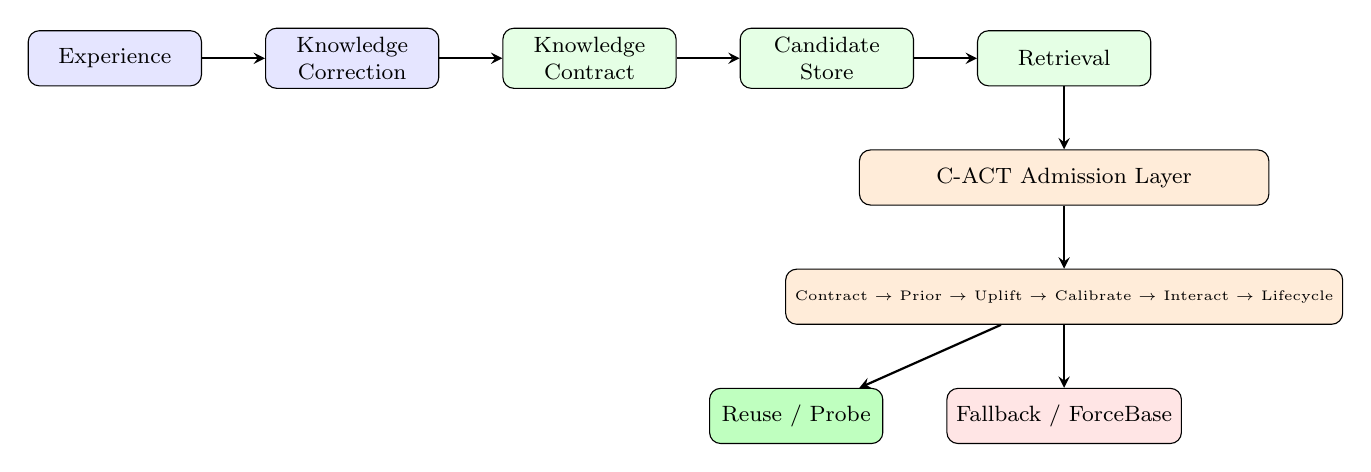
\begin{tikzpicture}[
    node distance=8mm,
    box/.style={rectangle, draw, rounded corners, minimum width=22mm, minimum height=7mm, align=center, font=\footnotesize},
    arrow/.style={->, >=stealth, thick}
]
\node[box, fill=blue!10] (exp) {Experience};
\node[box, fill=blue!10, right=of exp] (corr) {Knowledge\\Correction};
\node[box, fill=green!10, right=of corr] (contract) {Knowledge\\Contract};
\node[box, fill=green!10, right=of contract] (store) {Candidate\\Store};
\node[box, fill=green!10, right=of store] (retrieval) {Retrieval};
\node[box, fill=orange!15, below=of retrieval, minimum width=52mm] (admission) {C-ACT Admission Layer};
\node[box, fill=orange!15, below=of admission, minimum width=52mm, font=\tiny] (detail) {Contract $\rightarrow$ Prior $\rightarrow$ Uplift $\rightarrow$ Calibrate $\rightarrow$ Interact $\rightarrow$ Lifecycle};
\node[box, fill=red!10, below=of detail] (reject) {Fallback / ForceBase};
\node[box, fill=green!25, left=of reject] (accept) {Reuse / Probe};

\draw[arrow] (exp) -- (corr);
\draw[arrow] (corr) -- (contract);
\draw[arrow] (contract) -- (store);
\draw[arrow] (store) -- (retrieval);
\draw[arrow] (retrieval) -- (admission);
\draw[arrow] (admission) -- (detail);
\draw[arrow] (detail) -- (accept);
\draw[arrow] (detail) -- (reject);
\end{tikzpicture}
\caption{\textsc{C-ACT} system architecture. Experience-corrected knowledge is wrapped in a Knowledge Contract, stored, retrieved, and passes through the admission layer.}
\label{fig:architecture}
\end{figure}

\subsection{Knowledge Contract}

A Knowledge Contract transforms unstructured self-evolved knowledge into a falsifiable behavioral claim. Formally, a contract $u$ is a structured record:

\begin{align}
u = (& \text{knowledge\_id}, \; \text{type}, \; \text{level}, \; \text{gene}, \; \text{full\_text}, \nonumber\\
     & \text{claimed\_context}, \; \text{preconditions}, \; \text{postconditions}, \nonumber\\
     & \text{expected\_uplift}, \; \text{risk\_bound}, \; \text{non\_applicable\_contexts}, \; \text{status})
\end{align}

Knowledge types include \texttt{skill}, \texttt{remedy}, \texttt{dependency\_correction}, \texttt{action\_correction}, and \texttt{failure\_memory}. Levels (\texttt{strategy}, \texttt{functional}, \texttt{atomic}, \texttt{dependency}, \texttt{failure\_memory}) determine prior strength and risk standards.

Preconditions and postconditions are evaluated by a \texttt{ContractChecker}. Precondition evaluation supports three pattern types: exact match (\texttt{target\_block == diamond\_ore}), set membership (\texttt{current\_tool in \{iron\_pickaxe, diamond\_pickaxe\}}), and set exclusion (\texttt{current\_tool not in \{stone\_pickaxe, wooden\_pickaxe\}}). Binary existence checks (\texttt{has\_furnace}) and hard safety flags are also supported.

\textbf{Hard safety boundaries} are encoded in \texttt{non\_applicable\_contexts}---a list of contexts where reuse is unconditionally forbidden: \texttt{lava\_nearby}, \texttt{low\_health} (HP $< 5$), \texttt{combat}, \texttt{near\_cliff}, \texttt{irreversible\_resource\_constraint}. These are enforced \emph{before} any statistical gate evaluation.

\subsection{TrustStore: Three Beta Posteriors}

For each $(u, c)$ pair---knowledge item $u$ in context bucket $c$---\textsc{C-ACT} maintains three independent Beta posteriors:

\begin{align}
p_{\text{use}}(u, c) &\sim \text{Beta}(\alpha_{\text{use}}, \beta_{\text{use}}) \\
p_{\text{base}}(u, c) &\sim \text{Beta}(\alpha_{\text{base}}, \beta_{\text{base}}) \\
p_{\text{harm}}(u, c) &\sim \text{Beta}(\alpha_{\text{harm}}, \beta_{\text{harm}})
\end{align}

The \texttt{use} posterior tracks success probability when knowledge is actually reused. The \texttt{base} posterior tracks success probability when the agent uses its fallback policy instead---this is the control condition for counterfactual comparison. The \texttt{harm} posterior tracks the probability of harmful outcomes.

\textbf{Context bucket encoding.} Contexts are encoded into bucket keys for statistical sharing: \texttt{knowledge\_type | subgoal\_type | failure\_type | inventory\_sig | risk\_level | task\_tier}. A ContextBucket component supports adaptive split/merge based on within-bucket calibration error (ECE $> 0.15$ triggers split; KL divergence $< 0.05$ triggers merge).

\textbf{Active base logging.} To estimate $p_{\text{base}}$, \textsc{C-ACT} randomly forces 5--30\% of reuse-eligible decisions to use the base policy instead. The force probability adapts to three factors: uncertainty ($U = 4\pi(1-\pi)$), sample imbalance ($B = |n_{\text{use}} / (n_{\text{use}} + n_{\text{base}}) - 0.5|$), and danger level. The formula is:

\begin{equation}
q_{\text{base}}(u,c) = \text{clip}(q_{\min} + a \cdot U + b \cdot B - d \cdot \text{Danger}(c), \; 0.05, \; 0.30)
\end{equation}

High-danger contexts receive near-zero force probability, ensuring active logging never endangers the agent. Every forced-base decision records its propensity for inverse-propensity weighting.

\textbf{Empirical Bayes priors.} Rather than hand-tuned priors, \textsc{C-ACT} estimates level-aware priors from historical data using method-of-moments, with shrinkage toward a global prior:

\begin{equation}
\text{Prior}_{z,l} = w_{z,l} \cdot \text{Prior}_{z,l}^{\text{emp}} + (1 - w_{z,l}) \cdot \text{Prior}_{\text{global}}, \quad w_{z,l} = \min\left(\frac{n_{z,l}}{n_{z,l} + 20}, \; 0.8\right)
\end{equation}

where $n_{z,l}$ is the number of observations for knowledge type $z$ at level $l$.

\subsection{Bayesian Counterfactual Uplift}

The core decision statistic is the posterior probability that reusing knowledge $u$ improves outcomes:

\begin{equation}
\boxed{\pi_u(c) = P(p_{\text{use}} > p_{\text{base}} + \delta_{g,l}^\star \mid \mathcal{D})}
\end{equation}

This is computed exactly via the Beta-Binomial integral using the log-Beta function for numerical stability. The safety metric is the 95\% posterior upper bound on harmful reuse:

\begin{equation}
h_u^+(c) = Q_{0.95}[p_{\text{harm}}]
\end{equation}

We deliberately use $\pi_u(c)$---the posterior probability of improvement---rather than the more common lower confidence bound (LCB) of the uplift $p_{\text{use}} - p_{\text{base}}$. The LCB can be negative even when the posterior probability of improvement is high (e.g., with wide but right-skewed posteriors). $\pi_u(c)$ directly answers the question the gate needs: ``how confident are we that this helps?''

\subsection{Adaptive Calibration}

Rather than hand-tuning thresholds, \textsc{C-ACT} calibrates per-group parameters from a held-out calibration set:

\begin{equation}
\lambda^\star = \arg\max_{\lambda} \; \text{Coverage}(\lambda) \quad \text{s.t.} \quad \text{Risk}^+(\lambda) \leq \epsilon_{\text{harm}}
\end{equation}

where $\lambda = (\tau_{g,l}, \delta_{g,l}, h_{g,l}, \theta_{\text{int}})$ are the uplift probability threshold, minimum effect size, harm bound, and interaction threshold for task group $g$ and knowledge level $l$. Only $\epsilon_{\text{harm}} = 0.10$ is fixed a priori. The search space is discrete: $\tau \in \{0.80, 0.85, 0.88, 0.90, 0.92, 0.95\}$, $\delta \in \{0.02, 0.03, 0.05, 0.08, 0.10\}$, $h \in \{0.06, 0.08, 0.10, 0.12, 0.15\}$ (150 candidates per group).

Coverage and risk are computed on the calibration set:

\begin{align}
\text{Coverage}(\lambda) &= \frac{\#\text{allowed reuse}}{\#\text{candidate reuse}}, \quad
\text{Risk}^+(\lambda) = Q_{0.90}[\text{Beta}(k+1, n-k+1)]
\end{align}

where $k = \#\text{harmful allowed}$ and $n = \#\text{allowed}$. The 90\% binomial upper confidence bound ensures finite-sample safety.

\textbf{Task groups:} \texttt{crafting}, \texttt{mining}, \texttt{exploration}, \texttt{tech\_tree}, \texttt{failure\_recovery}, \texttt{interaction\_stress}.

\subsection{Four-Condition Admission Gate}

Knowledge $u$ is permitted in context $c$ iff all four conditions hold:

\begin{equation}
\boxed{
\text{admit}(u,c) \Longleftrightarrow
\underbrace{\pi_u(c) \ge \tau_{g,l}^\star}_{\text{Uplift}}
\;\land\;
\underbrace{h_u^+(c) \le h_{g,l}^\star}_{\text{Harm}}
\;\land\;
\underbrace{\text{ContractSatisfied}(u,c)}_{\text{Pre/Post}}
\;\land\;
\underbrace{\text{InteractionSafe}(u, \mathcal{P}, c)}_{\text{Pairwise}}
}
\end{equation}

\textbf{Cold-start handling.} When effective sample size (ESS) $= n_{\text{use}} + n_{\text{base}} + n_{\text{harm}} < n_{\min}$, the gate is supplemented by \textbf{safe Thompson probing}: with adaptive probability, we sample from the joint Beta posteriors and admit knowledge if all three sampled values satisfy the gate. This breaks the cold-start deadlock (no data $\rightarrow$ never admit $\rightarrow$ never get data) while respecting safety constraints.

\subsection{Interaction-Aware Reuse}

When multiple knowledge items are reused simultaneously, \textsc{C-ACT} checks pairwise interactions. For items $u_i, u_j$:

\begin{equation}
\Delta_{\text{int}}(u_i, u_j, c) = \Delta(u_i \land u_j, c) - \Delta(u_i, c) - \Delta(u_j, c)
\end{equation}

Pairs are classified into five states based on joint posterior evidence: synergy (allow, boost 1.05$\times$), neutral (allow), conflict (block pair), unknown-low-risk (allow with logging), and unknown-high-risk (force fallback). Conflict pairs are replaced with the single best-scoring certified item.

\subsection{Knowledge Lifecycle with Supervised Reuse}

Knowledge transitions through six states based on accumulating evidence:

\begin{center}
\fbox{\texttt{Candidate} $\xrightarrow{\text{contract}}$ \texttt{Quarantined} $\xrightarrow{n \ge 3, \pi_u > 0.3}$ \texttt{Probation} $\xrightarrow{n \ge 5, \pi_u \ge \tau^\star, h^+ \le h^\star}$ \texttt{Certified} $\xrightarrow{\text{violations}}$ \texttt{Deprecated} $\xrightarrow{\text{repeated}}$ \texttt{Disabled}}
\end{center}

\textbf{Supervised reuse} is the critical innovation. Probation-phase knowledge has 3--5 observations---enough to suggest benefit but with wide posteriors. Rather than blocking all Probation knowledge (false negatives) or granting unrestricted access (harm risk), \textsc{C-ACT} permits supervised reuse: the knowledge is used, but every execution step triggers an immediate reflection check. Failure triggers fallback. Only \texttt{Certified} knowledge enjoys unrestricted reuse.

\textbf{Temporal decay} shrinks posteriors toward priors at rate $\rho^{\Delta t}$ with adaptive $\rho \in [0.85, 0.99]$. $\rho$ decreases when recent prediction error exceeds 0.3 (faster forgetting under drift) and increases when error is below 0.1 (stable retention).

\subsection{Algorithm Summary}

\begin{algorithm}[t]
\caption{\textsc{C-ACT} Admission Decision}
\label{alg:cact}
\begin{algorithmic}[1]
\REQUIRE Candidate set $\mathcal{R}$, state $s$, context $c$, mode $m$
\ENSURE Decision $\in$ \{reuse, fallback, probe, force\_base\}
\STATE $\mathcal{V} \gets \emptyset$
\FOR{$u \in \mathcal{R}$}
    \IF{$\neg$ContextMatch$(u,c)$ $\lor$ $\neg$Preconditions$(u,s)$ $\lor$ NonApplicable$(u,s)$}
        \STATE \textbf{continue}
    \ENDIF
    \STATE $\mathcal{V} \gets \mathcal{V} \cup \{u\}$
\ENDFOR
\IF{$\mathcal{V} = \emptyset$} \RETURN (fallback, $\emptyset$) \ENDIF
\STATE DecayAll()
\FOR{$u \in \mathcal{V}$}
    \STATE $\pi_u \gets P(p_{\text{use}} > p_{\text{base}} + \delta_{g,l} \mid \mathcal{D})$
    \STATE $h_u^+ \gets Q_{0.95}[p_{\text{harm}}]$
    \STATE $\text{cert}_u \gets (\pi_u \ge \tau_{g,l}) \land (h_u^+ \le h_{g,l})$
\ENDFOR
\STATE Sort $\mathcal{V}$ by $\pi_u$ descending
\STATE (safe, combos) $\gets$ InteractionCheck($\mathcal{V}$, $c$)
\FOR{$(u_i, u_j) \in$ combos.synergy}
    \STATE $\pi_{u_i}, \pi_{u_j} \gets \min(1.0, 1.05\cdot\pi_{u_i}), \min(1.0, 1.05\cdot\pi_{u_j})$
\ENDFOR
\FOR{$u \in \mathcal{V}$ by $\pi_u$ desc}
    \IF{$\text{cert}_u \land$ InteractionSafe($u$)}
        \STATE supervised $\gets$ ($u$.lifecycle = Probation)
        \RETURN (reuse, $u$, supervised)
    \ENDIF
\ENDFOR
\IF{$m \neq$ evaluation}
    \STATE w.p.\ $q_{\text{base}}$: \RETURN (force\_base, $\emptyset$)
    \STATE Thompson probe if ESS $< n_{\min}$ and safe
\ENDIF
\RETURN (fallback, $\emptyset$)
\end{algorithmic}
\end{algorithm}

\section{Experimental Setup}

\subsection{Base Agent and Implementation}

We instantiate \textsc{C-ACT} on a Minecraft agent using a Qwen2.5-VL-7B-Instruct VLM for planning and reflection, with a Steve-1 action model~\cite{lifshitz2023} for low-level control. The base agent accumulates experience-corrected knowledge through two mechanisms: dependency graph corrections (correcting item-to-item prerequisites) and action memory corrections (recording action-level fixes with typed failure feedback). The agent's knowledge is not standard skill text---it is structured dependency and action corrections, allowing evaluation of whether \textsc{C-ACT} operates beyond skill-library settings.

\textsc{C-ACT} is implemented in approximately 3,100 lines of Python (14 modules) with no additional GPU requirements beyond the base agent. The admission gate adds negligible latency ($<1$ms per decision) compared to VLM inference times (2--5s per call).

\subsection{Compared Methods}

We compare seven decision methods, from no gate to full \textsc{C-ACT}:

\begin{enumerate}
    \item \textbf{NoKnowledge}: Pure LLM planner, no knowledge base. Lower bound.
    \item \textbf{Base-NoGate}: Retrieve all relevant knowledge and reuse unconditionally---the default in most self-evolving agents.
    \item \textbf{BankCuration}: Relevance-based retrieval with merge/prune curation.
    \item \textbf{LifecycleSuccessGate}: Six-state lifecycle gating on mean success rate only ($\ge 0.5$). Ablates the Bayesian component.
    \item \textbf{FixedBayes}: Bayesian uplift with hand-tuned fixed thresholds ($\tau{=}0.90$, $\delta{=}0.05$, $h{=}0.10$). No adaptive calibration, no contract layer.
    \item \textbf{ACT}: Full \textsc{C-ACT} without the Knowledge Contract layer. Bayesian uplift, adaptive calibration, interaction checking, lifecycle governance; no precondition checking or hard safety boundaries. Isolates the contract contribution.
    \item \textbf{\textsc{C-ACT}-Full}: Complete system with all seven components.
\end{enumerate}

All methods share identical backbone, task sets, seeds, and environment interaction budgets.

\subsection{Tasks and Protocol}

Tasks are drawn from MCU-turbo~\cite{mcu2024} and MineDojo~\cite{minedojo2022}, organized into six groups: Crafting (8), Mining (7), Exploration (6), Long-Horizon/Tech Tree (7), Failure Recovery (4), and Interaction Stress (4)---36 total.

\textbf{E0 (Sanity):} Verify base agent, wrappers, logging (24 episodes).

\textbf{E1 (Accumulation):} Generate knowledge with active base logging (192 episodes).

\textbf{E2 (Calibration):} Learn per-group thresholds from held-out set (96--144 episodes).

\textbf{E3 (Main Evaluation):} Strict frozen---no test-time learning, no posterior updates, no new knowledge, no active logging, no Thompson probing. 36 tasks $\times$ 8 seeds $\times$ 7 methods = 2,016 episodes.

\textbf{E4 (Ablation):} Remove each component independently. 12 tasks $\times$ 5 seeds $\times$ 8 variants = 480 episodes.

\textbf{E5 (Online Evolution):} Five rounds of accumulation $\rightarrow$ calibration $\rightarrow$ frozen test. 3 methods $\times$ 5 rounds = 720 episodes.

\subsection{Metrics}

\begin{itemize}
    \item \textbf{SR} (Success Rate), \textbf{HardSR} (hard tasks only)
    \item \textbf{HRR} (Harmful Reuse Rate): fraction of reuse decisions causing progress regression or unrecoverable failure
    \item \textbf{KUS} (Knowledge Usage Success): $P(\text{success} \mid \text{reused})$
    \item \textbf{Coverage@Risk$\le$10\%}: max coverage while keeping 90\% binomial UCB of harm risk $\le$ 10\%
    \item \textbf{KPR} (Knowledge Pollution Rate): fraction of certified knowledge later deprecated for harm
\end{itemize}

Wilson 95\% CI for proportions, paired bootstrap for continuous metrics, hierarchical bootstrap over tasks and seeds. Manual audit of 10\% failure episodes.

\section{Results}

\boxed{\textbf{ALL NUMBERS BELOW ARE PLACEHOLDERS. Real results will replace them after experiments complete.}}

\begin{table}[t]
\centering
\caption{Main evaluation results (PLACEHOLDER VALUES).}
\label{tab:main}
\begin{tabular}{lccccc}
\toprule
\textbf{Method} & \textbf{SR} & \textbf{HardSR} & \textbf{HRR} & \textbf{Cov@R10\%} & \textbf{KUS} \\
\midrule
NoKnowledge         & [TBD] & [TBD] & ---   & ---   & ---   \\
Base-NoGate         & [TBD] & [TBD] & [TBD] & ---   & [TBD] \\
BankCuration        & [TBD] & [TBD] & [TBD] & [TBD] & [TBD] \\
LifecycleSuccessGate& [TBD] & [TBD] & [TBD] & [TBD] & [TBD] \\
FixedBayes          & [TBD] & [TBD] & [TBD] & [TBD] & [TBD] \\
ACT                 & [TBD] & [TBD] & [TBD] & [TBD] & [TBD] \\
\textbf{C-ACT-Full} & [TBD] & [TBD] & [TBD] & [TBD] & [TBD] \\
\bottomrule
\end{tabular}
\end{table}

\begin{table}[t]
\centering
\caption{Per-group SR for key methods (PLACEHOLDER VALUES).}
\label{tab:bygroup}
\begin{tabular}{lcccccc}
\toprule
\textbf{Method} & \textbf{Craft} & \textbf{Mine} & \textbf{Explore} & \textbf{Tech} & \textbf{FailRec} & \textbf{Inter} \\
\midrule
FixedBayes      & [TBD] & [TBD] & [TBD] & [TBD] & [TBD] & [TBD] \\
ACT             & [TBD] & [TBD] & [TBD] & [TBD] & [TBD] & [TBD] \\
\textbf{C-ACT}  & [TBD] & [TBD] & [TBD] & [TBD] & [TBD] & [TBD] \\
\bottomrule
\end{tabular}
\end{table}

\begin{table}[t]
\centering
\caption{Ablation results (PLACEHOLDER VALUES).}
\label{tab:ablation}
\begin{tabular}{lcccc}
\toprule
\textbf{Variant} & \textbf{SR} & \textbf{HRR} & \textbf{Cov@R10\%} \\
\midrule
C-ACT Full          & [TBD] & [TBD] & [TBD] \\
w/o Contract        & [TBD] & [TBD] & [TBD] \\
w/o Adaptive $\tau$ & [TBD] & [TBD] & [TBD] \\
w/o Active Calib    & [TBD] & [TBD] & [TBD] \\
w/o Lifecycle       & [TBD] & [TBD] & [TBD] \\
w/o Level Prior     & [TBD] & [TBD] & [TBD] \\
w/o Interaction     & [TBD] & [TBD] & [TBD] \\
w/o Thompson        & [TBD] & [TBD] & [TBD] \\
\bottomrule
\end{tabular}
\end{table}

\begin{table}[t]
\centering
\caption{Online evolution over 5 rounds (PLACEHOLDER VALUES).}
\label{tab:online}
\begin{tabular}{lccccc}
\toprule
\textbf{Method} & \textbf{R1 SR} & \textbf{R3 SR} & \textbf{R5 SR} & \textbf{KPR} \\
\midrule
Online-NoGate       & [TBD] & [TBD] & [TBD] & [TBD] \\
Online-BankCuration & [TBD] & [TBD] & [TBD] & [TBD] \\
Online-C-ACT        & [TBD] & [TBD] & [TBD] & [TBD] \\
\bottomrule
\end{tabular}
\end{table}

\subsection{Result Structure (to be filled post-experiment)}

The Results section will report: (1)~harmful reuse reduction (HRR) across methods, expected pattern of monotonic decrease from Base-NoGate through C-ACT-Full; (2)~coverage-risk calibration improvement from adaptive thresholds over FixedBayes; (3)~task success gains, expected concentrated on hard tasks (tech-tree, failure-recovery, interaction-stress) where knowledge reuse quality matters most, with null or minimal effect on exploration tasks (positive control); (4)~ablation component ranking; (5)~online evolution trends showing C-ACT preventing knowledge pollution while no-gate baselines degrade.

\section{Discussion}

\subsection{Why Admission Over Parameterization?}

A natural alternative would be to parameterize all candidate knowledge into model weights and rely on optimization to select useful knowledge. We argue this conflates \emph{representability} (can the model encode this knowledge?) with \emph{admissibility} (should it?). Parameterization without admission testing cannot distinguish knowledge that \emph{causes} success from knowledge that merely \emph{accompanies} it. In continual settings, admitting harmful parameter updates causes same-category forgetting that is expensive to reverse. \textsc{C-ACT}'s decision-time admission offers three advantages: (i)~reversibility---knowledge can be instantly disabled by lifecycle transition without retraining; (ii)~context-dependence---the same knowledge may be safe in one context and harmful in another; (iii)~auditability---contract verification and propensity logging provide a complete decision trace.

\subsection{Design Choices}

\textbf{Independent Beta posteriors.} We use independent Beta distributions rather than a joint Dirichlet model. This is deliberate: independent Betas are more robust under data sparsity, more computationally efficient ($O(1)$ conjugate updates), and more interpretable. The independence assumption is harmless because decisions only compare $p_{\text{use}}$ and $p_{\text{base}}$ through $\pi_u(c)$, which is well-defined regardless of their joint distribution.

\textbf{Probation as supervised reuse.} The key design choice in the lifecycle is giving Probation-phase knowledge conditional access rather than full reuse or full rejection. This shrinks the gate's false-negative rate---good knowledge contributes value during Probation---while preventing the wide-posterior risk that comes with unrestricted Certified access.

\subsection{Limitations}

\textbf{Contract extraction.} Current contract extraction uses keyword-based heuristics. While conservative (erring toward blocking), this can produce false-positive safety boundaries. Future work could use the VLM itself for higher-precision contract generation.

\textbf{Environment scope.} Our evaluation is in Minecraft. While Minecraft is arguably the most complex controllable open-world environment for agent research, validation in other settings would strengthen generality.

\textbf{Knowledge pipeline dependence.} \textsc{C-ACT} requires an upstream generation pipeline. It is purely an admission layer---it cannot create knowledge, only govern its reuse.

\section{Ethics Statement}

This work develops a decision-time governance mechanism for AI agents. \textsc{C-ACT} reduces harmful agent behavior (e.g., using the wrong tool for a dangerous operation, consuming irreplaceable resources) by enforcing contract-based safety boundaries and statistically calibrated risk budgets. The system is designed to make agent decisions more auditable through contract verification and propensity logging. We do not foresee direct negative societal impacts from this work; the primary risk is that a poorly calibrated gate could reject beneficial knowledge, reducing agent capability. This is mitigated by the supervised reuse regime and adaptive calibration. All experiments use simulated Minecraft environments; no real-world physical systems are involved.

\section{Conclusion}

We introduced \textsc{C-ACT}, a decision-time admission layer that addresses a structural gap in self-evolving agent design: the absence of causal measurement in knowledge reuse decisions. By transforming knowledge into falsifiable contracts, gating reuse on Bayesian counterfactual uplift with adaptively calibrated risk budgets, and governing knowledge through a six-state lifecycle with supervised reuse, \textsc{C-ACT} provides a principled framework for deciding whether retrieved knowledge should affect agent behavior. The system is lightweight, compatible with any knowledge generation pipeline, and fully auditable.

\bibliography{references}

\end{document}
